\begin{frame}{Where the Model Runs}

  {\centering
  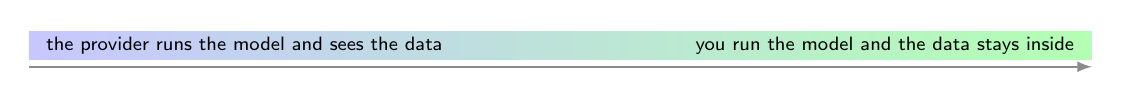
\begin{tikzpicture}[font=\sffamily\scriptsize, >=latex]
    \shade[left color=blue!22, right color=green!30] (0,0) rectangle (13.5,0.36);
    \draw[->, thick, black!45] (0,-0.09) -- (13.5,-0.09);
    \node[anchor=west] at (0.1,0.18) {the provider runs the model and sees the data};
    \node[anchor=east] at (13.4,0.18) {you run the model and the data stays inside};
  \end{tikzpicture}\\[0.25em]
  {\scriptsize\setlength{\tabcolsep}{3pt}
  \begin{tabular}{>{\raggedright\arraybackslash}p{2.05cm} *{5}{>{\raggedright\arraybackslash}p{2.05cm}}}
    \toprule
     & \textbf{Public API} & \textbf{Dedicated endpoint} & \textbf{Rented cloud GPUs} & \textbf{On-premises} & \textbf{Air-gapped} \\
    \midrule
    \textbf{Data processed by} & provider & provider (reserved for you) & you, on rented hardware & you & you \\
    \textbf{Operated by} & provider & provider & you & you & you \\
    \textbf{Models} & closed or open & closed or open & open-weight & mostly open-weight & mostly open-weight \\
    \textbf{Cost model} & per token & per reserved hour & per GPU-hour & fixed (owned) & fixed (owned) \\
    \bottomrule
  \end{tabular}\par}\par}
  \vspace{0.3em}
  \begin{itemize}\scriptsize\itemsep0.2em
    \item[\textcolor{red}{$\blacktriangleright$}] \textbf{On-premises:} the model runs on hardware you own, in your data centre. \textbf{Open-weight:} the trained weights are published, so anyone can run the model; closed models are usually reached through their provider's API.
    \item[\textcolor{red}{$\blacktriangleright$}] \textbf{Air-gapped:} on-premises with no network path to the outside. Weights, container images and packages arrive through an offline mirror, and outbound calls are switched off (\texttt{VLLM\_NO\_USAGE\_STATS=1}, \texttt{HF\_HUB\_OFFLINE=1}).
    \item[\textcolor{red}{$\blacktriangleright$}] \textbf{Who sees the prompts:} OpenAI's abuse-monitoring logs, which can hold API prompts and responses, are ``retained for up to 30 days'' by default. Only the last two columns keep every prompt in-house (see the privacy section of this lecture).
  \end{itemize}
  \vspace{0.1em}
  {\scriptsize OpenAI, ``Data controls in the OpenAI platform,'' accessed 6 Oct.\ 2026, \href{https://developers.openai.com/api/docs/guides/your-data}{developers.openai.com}; vLLM, ``Usage Stats Collection,'' \href{https://docs.vllm.ai/en/latest/usage/usage_stats/}{docs.vllm.ai}; Hugging Face, ``Environment variables,'' \href{https://huggingface.co/docs/huggingface_hub/package_reference/environment_variables}{huggingface.co/docs}.\par}
\end{frame}

\begin{frame}{The On-Premises Decision and Its Break-Even}
  \begin{columns}[T,onlytextwidth]
    \column{0.40\textwidth}
      {\footnotesize\textbf{Reasons to run it yourself}\par}
      \begin{itemize}\scriptsize\itemsep0.1em
        \item[\textcolor{red}{$\blacktriangleright$}] Prompts and documents stay inside the network.
        \item[\textcolor{red}{$\blacktriangleright$}] Low latency to internal systems.
        \item[\textcolor{red}{$\blacktriangleright$}] Per-department adapters, and a model that changes only when you promote a new version.
        \item[\textcolor{red}{$\blacktriangleright$}] No exposure to a provider's price changes or model retirements.
      \end{itemize}
      \vspace{0.2em}
      {\footnotesize\textbf{What it costs}\par}
      \begin{itemize}\scriptsize\itemsep0.1em
        \item[\textcolor{red}{$\blacktriangleright$}] An operations team: on-call, upgrades, security patches.
        \item[\textcolor{red}{$\blacktriangleright$}] The capability gap of open-weight models (next slide).
        \item[\textcolor{red}{$\blacktriangleright$}] Utilisation risk: an idle GPU costs as much as a busy one.
      \end{itemize}
      \vspace{0.2em}
      \begin{itemize}\scriptsize
        \item[\textcolor{red}{$\blacktriangleright$}] \textbf{Reading the table:} against a hosted copy of the same model, owning pays only at 44\% of full-load throughput around the clock, which working-hours traffic rarely sustains. Against a frontier API the bar is 4\%, for a weaker model.
      \end{itemize}
    \column{0.58\textwidth}
      \begin{itemize}\scriptsize\itemsep0.2em
        \item[\textcolor{red}{$\blacktriangleright$}] \textbf{Break-even volume} $V^{*}$: the monthly number of generated tokens at which API spend equals the fixed cost of owning,
          \[ \frac{p\,V^{*}}{10^{6}} = F \quad\Longrightarrow\quad V^{*} = \frac{10^{6}\,F}{p}, \]
          with $p$ the API cost per million generated tokens (input-token charges included) and $F$ the monthly cost of owned hardware (amortised), power, space and staff.
        \item[\textcolor{red}{$\blacktriangleright$}] \textbf{Capacity check:} with throughput $T$ in generated tokens/s and $s \approx 2.6\times10^{6}$ seconds per month, the hardware must run at \textbf{utilisation} $u^{*} = V^{*}/(T s)$, the fraction of the month at throughput $T$.
        \item[\textcolor{red}{$\blacktriangleright$}] \textbf{Example:} an 8-GPU H100 server running Llama 3.3 70B in FP8 as four 2-GPU replicas (1,000 tokens in, 1,000 out) generates $T = 8 \times 2{,}209 = 17{,}672$ tokens/s at full load, so $T s \approx 4.59\times10^{10}$ tokens per month. Assume $F = \$20{,}000$ per month.
      \end{itemize}
      {\centering\scriptsize\setlength{\tabcolsep}{3pt}
      \begin{tabular}{l r r r}
        \toprule
        \textbf{Alternative} & $p$ (assumed) & $V^{*}$ per month & $u^{*}$ \\
        \midrule
        same model, hosted & \$1 & $2.0\times10^{10}$ & 0.44 \\
        frontier closed API & \$10 & $2.0\times10^{9}$ & 0.04 \\
        \bottomrule
      \end{tabular}\par}
  \end{columns}
  \vspace{0.2em}
  {\scriptsize $T$: NVIDIA, TensorRT-LLM performance overview (Llama 3.3 70B, FP8, H100, two GPUs per replica), updated 26 Sep.\ 2026, \href{https://nvidia.github.io/TensorRT-LLM/developer-guide/perf-overview.html}{nvidia.github.io/TensorRT-LLM}. $F$ and $p$ are illustrative assumptions.\par}
\end{frame}

\begin{frame}{Choosing an Open-Weight Model}
  \begin{itemize}\scriptsize\itemsep0.2em
    \item[\textcolor{red}{$\blacktriangleright$}] \textbf{The gap:} from January to May 2026 the most capable open-weight models trailed frontier closed models by four months on average, 8 points on Epoch AI's Epoch Capabilities Index (ECI, a composite of many benchmarks). Open models ``tend to perform worse on private benchmarks'', so this may understate the gap.
    \item[\textcolor{red}{$\blacktriangleright$}] \textbf{Language support differs by model:} on Arabic MMMLU (MMLU professionally translated into 14 languages), gpt-oss-120b scores 82.7 against 90.4 for OpenAI's closed o3. Llama 3.3 supports eight languages, Arabic not among them; the released ALLaM-7B was trained from scratch on English, then on Arabic and English.
    \item[\textcolor{red}{$\blacktriangleright$}] \textbf{Procedure:} shortlist on public benchmarks, decide on your own evaluation set (covered earlier), then check the columns below. For mixture-of-experts models (covered earlier), memory follows total parameters and per-token compute follows active ones.
  \end{itemize}
  \vspace{0.1em}
  {\centering\scriptsize\setlength{\tabcolsep}{3pt}
  \begin{tabular}{>{\raggedright\arraybackslash}p{2.9cm} >{\raggedright\arraybackslash}p{1.8cm} >{\raggedright\arraybackslash}p{1.2cm} >{\raggedright\arraybackslash}p{3.2cm} >{\raggedright\arraybackslash}p{3.6cm}}
    \toprule
    \textbf{Model (year)} & \textbf{Total / active parameters} & \textbf{Context (tokens)} & \textbf{Licence} & \textbf{Weights as served} \\
    \midrule
    Qwen3.8-27B (2026) & 27B dense & 262,144 & Apache 2.0 & 56\,GB in \texttt{bf16}: one GPU \\
    Llama 3.3 70B (2024) & 70B dense & 131,072 & Llama 3.3 Community License & 141\,GB in \texttt{bf16}; 40\,GB at 4 bits \\
    gpt-oss-120b (2025) & 117B / 5.1B & 131,072 & Apache 2.0 & experts in MXFP4 (4.25 bits per weight): one 80\,GB GPU \\
    Qwen3.8-2.4T-A95B (2026) & 2.4T / 95B & 262,144 & custom Qwen licence & 4.9\,TB in \texttt{bf16}: eight nodes of 8 $\times$ 80\,GB \\
    \bottomrule
  \end{tabular}\par}
  \vspace{0.2em}
  {\scriptsize Edwards and Emberson, ``Open models lag state-of-the-art closed models by 4 months,'' Epoch AI, 29 May 2026, \href{https://epoch.ai/data-insights/open-closed-eci-gap}{epoch.ai}; OpenAI, ``gpt-oss-120b \& gpt-oss-20b Model Card,'' 2025, \href{https://arxiv.org/abs/2508.10925v1}{arXiv:2508.10925v1}, Table~2; model cards of Qwen3.8, Llama 3.3, ALLaM-7B.\par}
\end{frame}

\begin{frame}{A Reference Serving Stack}

  {\centering
  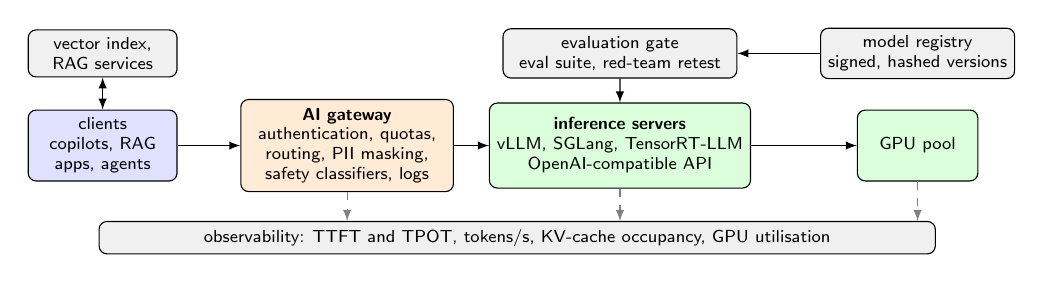
\begin{tikzpicture}[font=\sffamily\scriptsize, >=latex, scale=0.9,
      every node/.style={transform shape},
      box/.style={draw, rounded corners=0.1cm, align=center, inner sep=3pt},
      req/.style={box, fill=blue!12},
      gwy/.style={box, fill=orange!16},
      srv/.style={box, fill=green!14},
      side/.style={box, fill=gray!12}]
    \node[req, minimum width=2.1cm, minimum height=1.0cm] (cli) at (0,1.35) {clients\\copilots, RAG\\apps, agents};
    \node[gwy, minimum width=3.0cm, minimum height=1.3cm] (gw) at (3.45,1.35) {\textbf{AI gateway}\\authentication, quotas,\\routing, PII masking,\\safety classifiers, logs};
    \node[srv, minimum width=3.3cm, minimum height=1.2cm] (srv) at (7.3,1.35) {\textbf{inference servers}\\vLLM, SGLang, TensorRT-LLM\\OpenAI-compatible API};
    \node[srv, minimum width=1.7cm, minimum height=1.0cm] (gpu) at (11.5,1.35) {GPU pool};
    \node[side, minimum width=2.1cm] (rag) at (0,2.65) {vector index,\\RAG services};
    \node[side, minimum width=3.3cm] (gate) at (7.3,2.65) {evaluation gate\\eval suite, red-team retest};
    \node[side, minimum width=2.4cm] (reg) at (11.5,2.65) {model registry\\signed, hashed versions};
    \node[side, minimum width=11.8cm, minimum height=0.45cm] (obs) at (5.85,0.05) {observability: TTFT and TPOT, tokens/s, KV-cache occupancy, GPU utilisation};
    \draw[->] (cli) -- (gw);
    \draw[->] (gw) -- (srv);
    \draw[->] (srv) -- (gpu);
    \draw[<->] (cli) -- (rag);
    \draw[->] (reg) -- (gate);
    \draw[->] (gate) -- (srv);
    \draw[->, dashed, black!50] (gw.south) -- (gw.south |- obs.north);
    \draw[->, dashed, black!50] (srv.south) -- (srv.south |- obs.north);
    \draw[->, dashed, black!50] (gpu.south) -- (gpu.south |- obs.north);
  \end{tikzpicture}\\[0.1em]
  {\scriptsize Every request passes the gateway; weights reach the servers only from the model registry (covered earlier), through the evaluation gate.\par}\par}
  \vspace{0.2em}
  \begin{columns}[T,onlytextwidth]
    \column{0.48\textwidth}
      \begin{itemize}\scriptsize\itemsep0.15em
        \item[\textcolor{red}{$\blacktriangleright$}] \textbf{AI gateway:} the single entry point in front of every model (for example LiteLLM). It authenticates callers, enforces quotas, routes by model name, masks personally identifiable information (PII), runs the safety classifiers of the jailbreak-defenses section, and keeps logs for a set retention period. The governance practice covered earlier (review before release, incident reporting, a kill switch) is enforced here.
      \end{itemize}
    \column{0.50\textwidth}
      \begin{itemize}\scriptsize\itemsep0.15em
        \item[\textcolor{red}{$\blacktriangleright$}] \textbf{OpenAI-compatible API:} the HTTP interface of OpenAI's API (\texttt{/v1/chat/completions}). vLLM, SGLang and TensorRT-LLM all serve it, so engines and models change behind the gateway without client changes.
        \item[\textcolor{red}{$\blacktriangleright$}] \textbf{Model signing:} a signature over a manifest of every model file's SHA-256 hash, checked on import and at load, so tampered weights (data-poisoning section) are refused. OpenSSF Model Signing v1.0 also works with self-signed certificates or plain key pairs.
      \end{itemize}
  \end{columns}
  \vspace{0.1em}
  {\scriptsize OpenSSF, ``Launch of Model Signing v1.0,'' 4 Apr.\ 2025, \href{https://openssf.org/blog/2025/04/04/launch-of-model-signing-v1-0-openssf-ai-ml-working-group-secures-the-machine-learning-supply-chain/}{openssf.org}, and the OMS specification post, 25 Jun.\ 2025, \href{https://openssf.org/blog/2025/06/25/an-introduction-to-the-openssf-model-signing-oms-specification/}{openssf.org}; vLLM, SGLang, TensorRT-LLM and LiteLLM documentation.\par}
\end{frame}

\begin{frame}{Many Adapters on One Base Model}
  \begin{columns}[T,onlytextwidth]
    \column{0.50\textwidth}
      \begin{itemize}\scriptsize\itemsep0.25em
        \item[\textcolor{red}{$\blacktriangleright$}] \textbf{The problem:} per-department LoRA adapters (covered earlier; see the domain-specific LLMs section) share one base model. Merging each into its own copy of the weights multiplies memory: on one 80\,GB A100, S-LoRA's merged-copies baseline served 5 Llama-7B adapters and ran out of memory at 100, the next count tested.
        \item[\textcolor{red}{$\blacktriangleright$}] \textbf{Multi-LoRA serving} keeps one copy of the base weights and batches requests that name different adapters:
          \[ y_i = x_i W + x_i A_i B_i , \]
          $x_i$: input of request $i$; $W$: shared base weight (one large product for the batch); $A_i, B_i$: the rank-$r$ factors of request $i$'s adapter (a small product per request).
        \item[\textcolor{red}{$\blacktriangleright$}] \textbf{S-LoRA} keeps all adapters in host memory and copies those of running requests to the GPU, into one paged pool shared with the KV cache (\textbf{Unified Paging}). With 2,000 adapters it served 7.61 requests/s, against 8.05 with 5 (Llama-7B, rank 8).
      \end{itemize}
    \column{0.48\textwidth}
      {\centering
      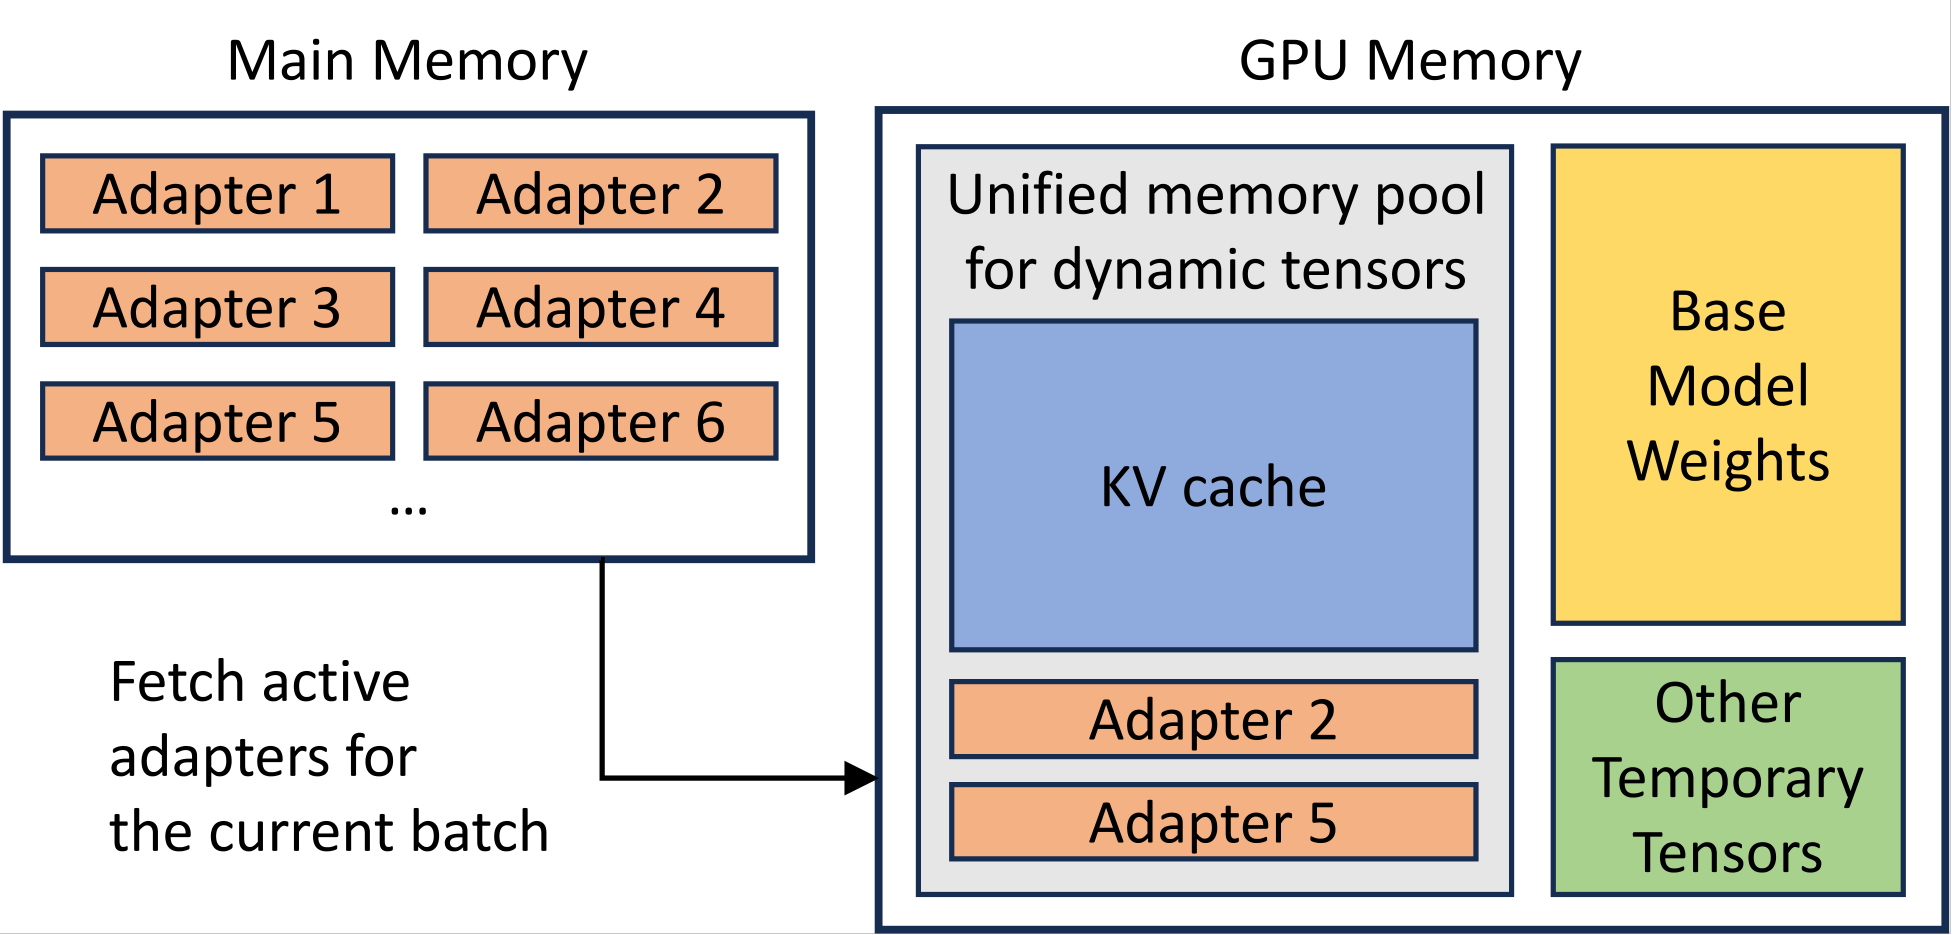
\includegraphics[width=\linewidth,height=0.32\textheight,keepaspectratio]{images/nlp-security-enterprise/slora_fig2_memory_allocation.png}\\[0.2em]
      {\scriptsize ``Overview of memory allocation in S-LoRA.'' Sheng et al., ``S-LoRA: Serving Thousands of Concurrent LoRA Adapters,'' MLSys 2024, \href{https://arxiv.org/abs/2311.03285v3}{arXiv:2311.03285v3}, Figure~2.\par}\par}
      \vspace{0.2em}
      \begin{itemize}\scriptsize\itemsep0.2em
        \item[\textcolor{red}{$\blacktriangleright$}] \textbf{Punica} batches all adapters with one kernel, SGMV (segmented gather matrix-vector multiplication): 12$\times$ the throughput of state-of-the-art serving systems, for 2\,ms of extra latency per token.
        \item[\textcolor{red}{$\blacktriangleright$}] vLLM (\texttt{-{}-enable-lora}) and SGLang serve adapters per request; the adapter is named in the API's \texttt{model} field, so the gateway routes each department to its own.
      \end{itemize}
  \end{columns}
  \vspace{0.1em}
  {\scriptsize Chen et al., ``Punica: Multi-Tenant LoRA Serving,'' MLSys 2024, \href{https://proceedings.mlsys.org/paper_files/paper/2024/hash/054de805fcceb78a201f5e9d53c85908-Abstract-Conference.html}{proceedings.mlsys.org}; vLLM, ``LoRA Adapters,'' \href{https://docs.vllm.ai/en/latest/features/lora/}{docs.vllm.ai}.\par}
\end{frame}

\begin{frame}{Fitting a 70B Model on One GPU}
  \begin{columns}[T,onlytextwidth]
    \column{0.44\textwidth}
      \begin{itemize}\scriptsize\itemsep0.3em
        \item[\textcolor{red}{$\blacktriangleright$}] Plain rounding to 4-bit weights (weight-only quantization, covered earlier) loses accuracy. Two error-aware post-training methods, both supported by vLLM:
        \item[\textcolor{red}{$\blacktriangleright$}] \textbf{GPTQ} quantizes column by column and updates the remaining weights to absorb each error, using the inverse Hessian (second derivatives of the layer's squared output error) from 128 calibration sequences. It brought 175B-parameter models to 3--4 bits in about four GPU hours.
        \item[\textcolor{red}{$\blacktriangleright$}] \textbf{AWQ} (activation-aware weight quantization) finds the 1\% salient weight channels from activation statistics and scales them up before rounding. It relies on no backpropagation or reconstruction (GPTQ's weight updates), so it does not overfit the calibration set.
        \item[\textcolor{red}{$\blacktriangleright$}] \textbf{Quality cost} (Llama-2-70B, 4 bits, groups of 128): WikiText-2 perplexity 3.32 in FP16, 3.46 with plain rounding, 3.42 with GPTQ, 3.41 with AWQ.
      \end{itemize}
    \column{0.54\textwidth}
      \begin{itemize}\scriptsize
        \item[\textcolor{red}{$\blacktriangleright$}] \textbf{Worked example:} the 70B grouped-query-attention model of the earlier 4-GPU example ($L = 80$, $n_{kv} = 8$, $d_{\text{head}} = 128$) needs 2.68\,GB of \texttt{bf16} KV cache per 8,192-token session (covered earlier). On one 80\,GB GPU:
      \end{itemize}
      {\centering\scriptsize\setlength{\tabcolsep}{3pt}
      \begin{tabular}{>{\raggedright\arraybackslash}p{6.0cm} r}
        \toprule
        \textbf{Item} & \textbf{GB} \\
        \midrule
        68.5B linear-layer weights, 0.5 byte each & 34.2 \\
        16-bit scale and 4-bit zero point per 128 weights & 1.3 \\
        embedding, output layer, norms in 16 bits (2.1B) & 4.2 \\
        \textbf{weights} (equal to the published AWQ checkpoint) & \textbf{39.8} \\
        per-GPU workspace of the 4-GPU example (assumed) & 5.0 \\
        \textbf{KV budget} $= 80 - 39.8 - 5$ & \textbf{35.2} \\
        \bottomrule
      \end{tabular}\par}
      \begin{itemize}\scriptsize\itemsep0.2em
        \item[\textcolor{red}{$\blacktriangleright$}] $35.2 / 2.68 \approx \mathbf{13}$ concurrent 8k sessions; about 26 with an 8-bit KV cache.
        \item[\textcolor{red}{$\blacktriangleright$}] Four such replicas on 4 GPUs hold about 52 sessions, against about 60 for one \texttt{bf16} replica sharded over 4 GPUs (covered earlier): a 4-bit copy (39.8\,GB) is larger than a quarter of the \texttt{bf16} weights (35\,GB). Four-bit weights buy a one-GPU entry point and replicas that fail independently.
      \end{itemize}
  \end{columns}
  \vspace{0.1em}
  {\scriptsize Frantar et al.\ (GPTQ), ICLR 2023, \href{https://arxiv.org/abs/2210.17323v2}{arXiv:2210.17323v2}; Lin et al.\ (AWQ), MLSys 2024, \href{https://arxiv.org/abs/2306.00978v5}{arXiv:2306.00978v5}, Table~4; checkpoint: \href{https://huggingface.co/hugging-quants/Meta-Llama-3.1-70B-Instruct-AWQ-INT4}{hugging-quants/Meta-Llama-3.1-70B-Instruct-AWQ-INT4}; vLLM, ``Quantization,'' \href{https://docs.vllm.ai/en/latest/features/quantization/}{docs.vllm.ai}.\par}
\end{frame}
